\chapter{Experimental Verification}
An initial experimental proof of principle experiment was performed at the SACLA FEL.
The experiments consisted of three parts: First, reproducing XXX and imaging projection of the focal volume of the FEL by using metal foils as samples, performing a measurement of the K$\alpha$  fluorescence and an reconstruction in the small angle regime. Second, moving the a smaller length scale and try to image nanoparticles. And Third, leaving the small angle regime and record the fluoresccne of a single crystal and perform a reciprocal space reconstruction.
\section{Sample Preparation}
As an nanoparticle sample, spherical iron oxide nanoparticles where chosen. To improve the number of detected fluorescence photons per FEL shot, the decision was made to have many particles many for each shot within the focus. This ensures a higher number of fluorescence photons recorded and basically eliminates the possibility of having shots without any particles inside the focus. 

Magnetite Nanoparticles coated with Oleic Acid dispersed in Toluene were bought from NN-Labs, inhibited Methylmethacrylate (MMA) and Etyhlhexylmethacrylate (EHMA)  (Sigma Aldrich) were filtered using a prefilled column to remove the Inhibitor,  2,2-azo-bis-isobutyrylnitrile (AIBN) (Sigma Aldrich) was used as thermally activated radical initiator as received. Polystyrene (Sigma Aldrich, MW XXX) was used as received. As solvents, Methanol, Toluene and Chloroform were used.
\subsection{Nanoparticles in Polystyrene Matrix}
The nanoparticles were precipitated with Methanol, centrifuged and redispersed in Chloroform at a concentration of 25\,mg/ml, whereas the weight of nanoparticles includes the weight of the oleic acid capping. Polystyrene was dissolved in Chloroform at a concentration of 250\,mg/ml and different volumes of the nanoparticles solution were added (to account for the different iron contents) to 5\,ml of the Polystyrene solution (see \fref{tab:samplePS}). After ensuring dispersion by strong sonication, fractions of XXX\,ul the solution were dropped onto glass slides and dried. After drying, the approximately 200\,um thick films were carefully removed from the glass slides.
As an iron containing control sample, 60mg FeCl3 and XXX Polystyrene were dissolved in 6ml acetone, sonicated and  fractions of XXX were dropped onto slowly spinning glass slides (XXX rpm for XX 5\,min) and carefully removed after drying.
\begin{table}[tp]
	\centering
	\caption{Nanoparticles in Polystyrene recipes}
	\label{tab:samplePS}
	\begin{tabular}{llll}
		\hline
	NP size&   Volume NP in CF &  Iron Concentration &Volume PS in CF    \\
		\hline
	  5\,nm&700 ul & & 5\,ml  \\  
	   10\,nm&  500 ul& &5\,ml  \\    
	   20\,nm &  425 ul& &5\,ml  \\  
	   	Control   &  & &5\,ml  \\  
		\hline
	\end{tabular}
\end{table}

\subsection{Nanoparticles in Poly(MMA/EHMA)  Matrix}
As a second nanoparticle in polymer sample, a AIBN initiated Poly(MMA/EHMA) polymerisation with magnetite nanoparticles was performed. 
The nanoparticle solution was concentrated to XXX in toluene by precipitation, centrifugation and redispersion. To account for the different iron concentration, to different amounts of the nanoparticle solution and additional toluene, 800\,ul of EHMA was added each (see \fref{tab:sampleCP}). After strong sonication to ensure dispersion, 3.2\,ml of MMA were added and the solution was bubbled with N$_2$ for 5\,min. To start the polymerisation, 20\,mg of AIBN were added and the solution was bubbled again with N$_2$  for 10\,min before heating it up to XXX using a water bath under weak sonication using a sonic bath. The mixture was kept at XXX for XXX.
The vials were uncapped and the polymer dried for 12h at XXX. The polymer was removed from the vials and cut into slices of approximatly XXX thickness using a slow spinning diamond saw.
As a control sample, the polymerisation was performed without any nanoparticles added.

\begin{table}[tp]
	\centering
	\caption{Nanoparticles in PMMA/EHMA recipes}
	\label{tab:sampleCP}
	\begin{tabular}{llllll}
		\hline
		NP size &NP in Toluene&Toluene & EHMA & MMA & AIBN \\
		\hline
		5\,nm& & &800\,ul&  3.2\,ml&   20\,mg    \\
		10\,nm& & &800\,ul&  3.2\,ml&   20\,mg    \\
		10\,nm& & &0\,ul&  4\,ml&   20\,mg    \\
		20\,nm& & &800\,ul&  3.2\,ml&   20\,mg    \\
			Control& & 1\,ml&800\,ul&  3.2\,ml&   20\,mg    \\
		\hline
	\end{tabular}
\end{table}

\subsection{Nanoparticle Sample Characterisation}
Before sample preparation, the iron oxide nanoparticles as received were diluted with Toluene, deposited on a silicon nitride membrane and imaged using a FEI Tecnai microscope  (see \fref{fig:tem}).  For each of the three nominal sizes, 3 different areas on the membrane were analyzed using ImageJ, resulting in mean radii of 8.3$\pm$1.7\,nm ("20\,nm") 4.1$\pm$0.8 \,nm	("10\,nm") 3.1$\pm$0.6\,nm ("5\,nm"). In the TEM images, the effect of the oleic acid ligands used to stabilize the nanoparticle dispersion  can be seen as the inter-particle distance.

\begin{figure}[tp]
	\centering
	\begin{subfigure}[b]{0.3\textwidth}
		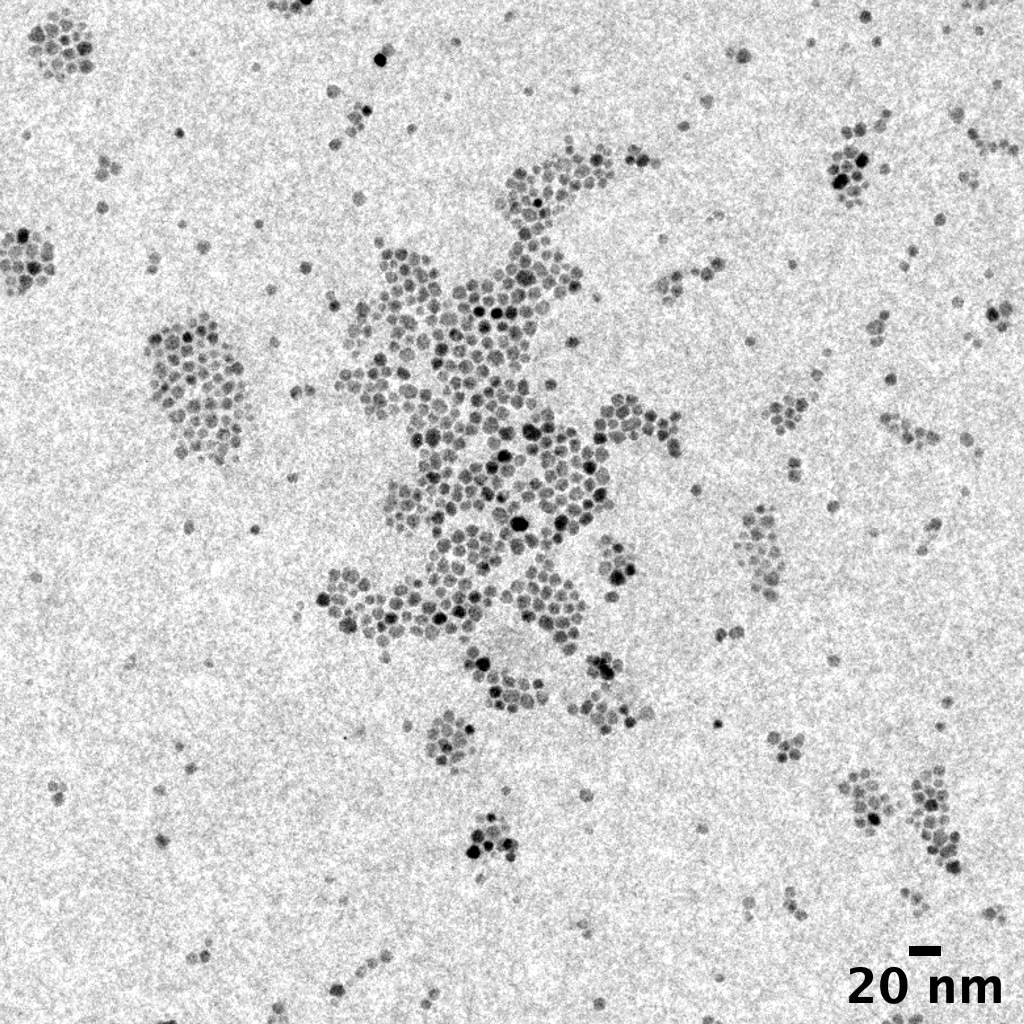
\includegraphics[width=\linewidth]{images/tem5.png}
	\end{subfigure}
	\begin{subfigure}[b]{0.3\textwidth}
		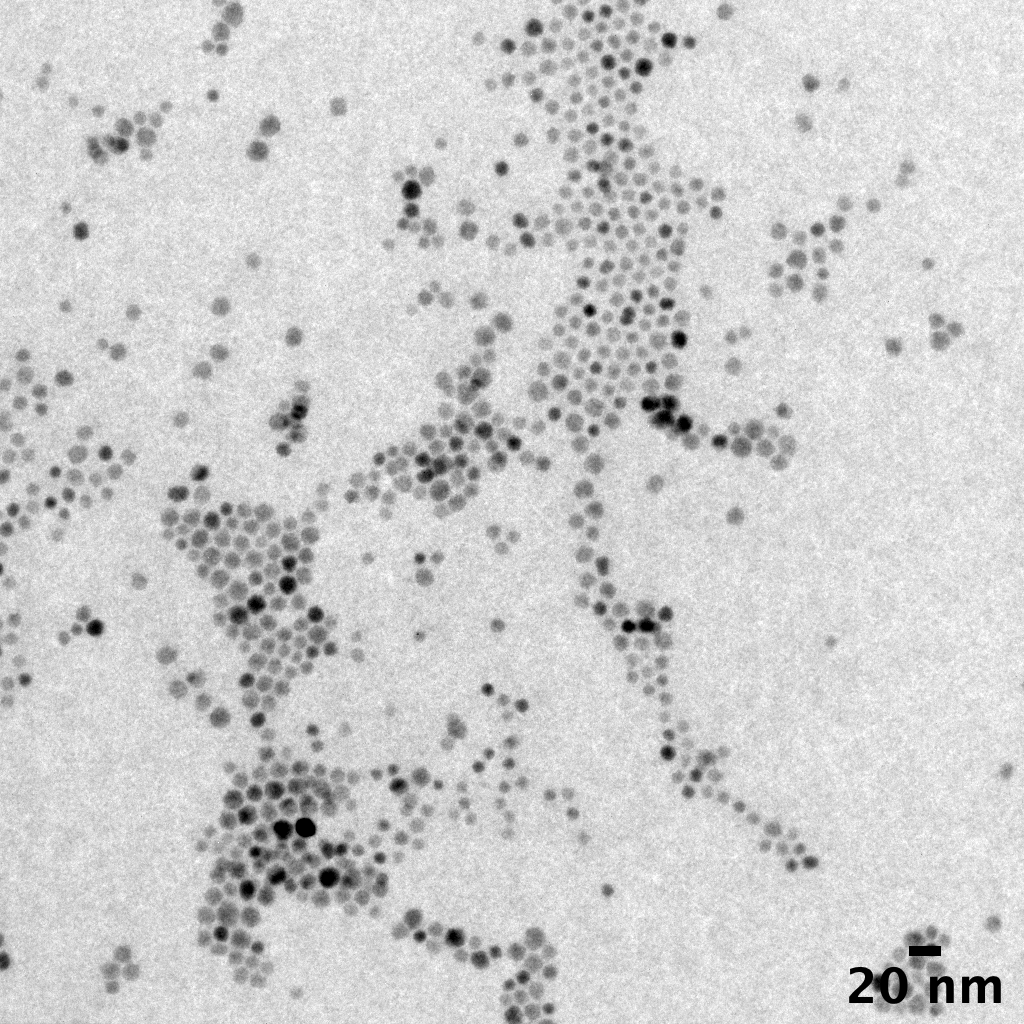
\includegraphics[width=\linewidth]{images/tem10.png}
	\end{subfigure}
	\begin{subfigure}[b]{0.3\textwidth}
		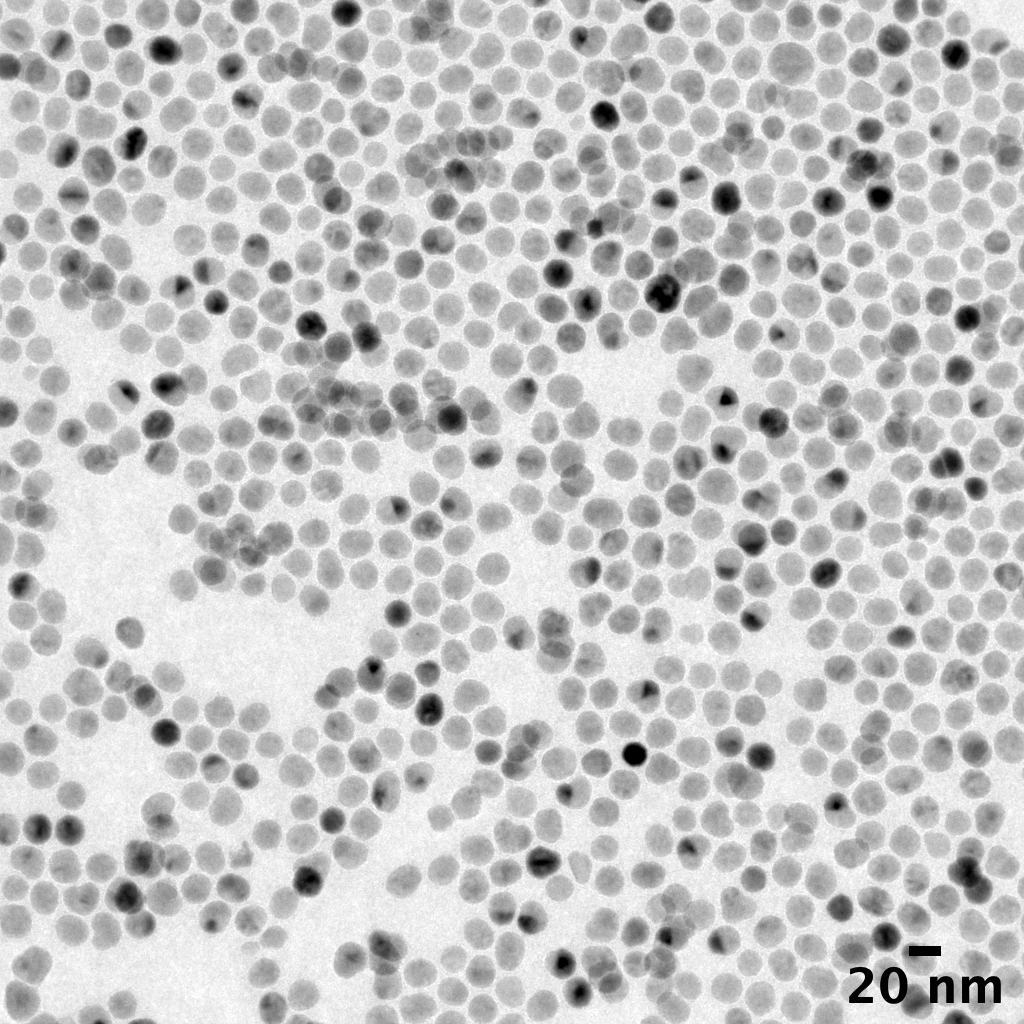
\includegraphics[width=\linewidth]{images/tem20.png}
	\end{subfigure}
\par\smallskip
	\begin{subfigure}[b]{0.3\textwidth}
		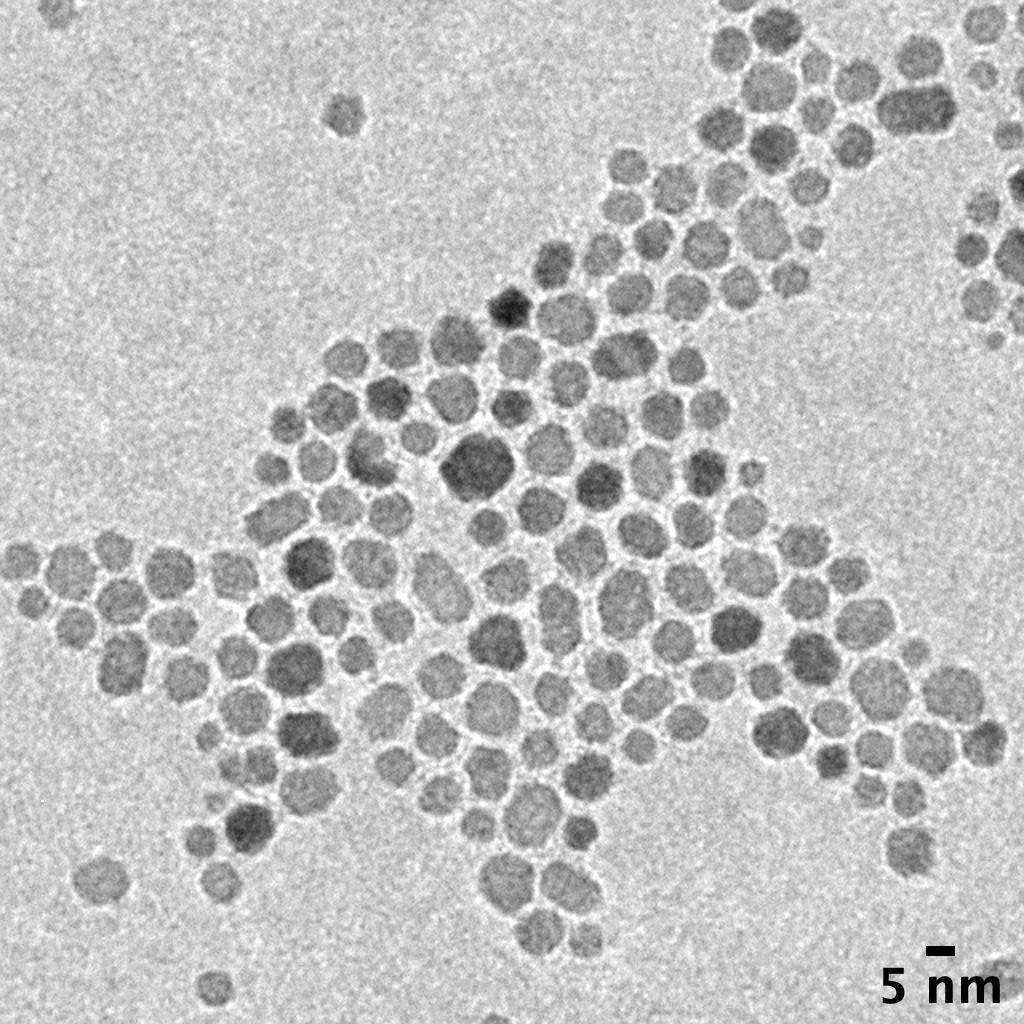
\includegraphics[width=\linewidth]{images/temh5.png}
	\end{subfigure}
	\begin{subfigure}[b]{0.3\textwidth}
		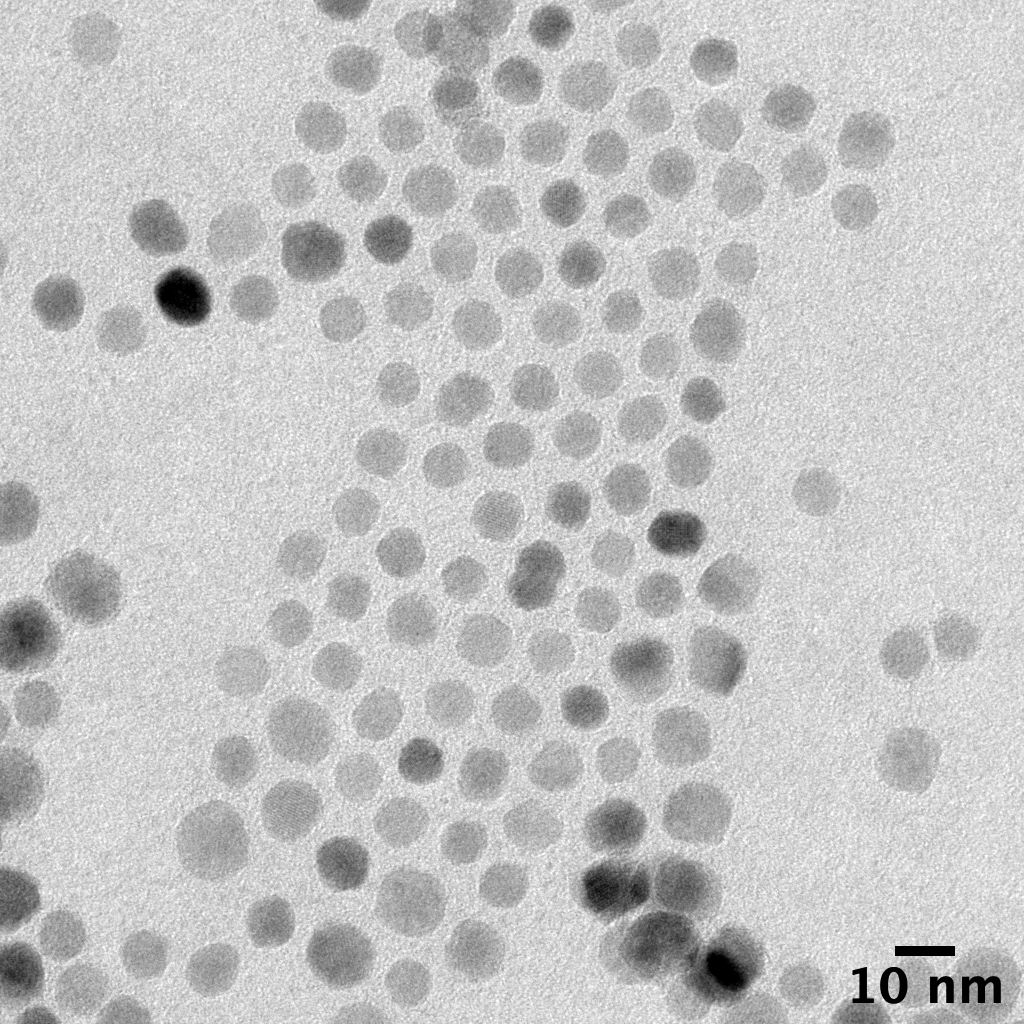
\includegraphics[width=\linewidth]{images/temh10.png}
	\end{subfigure}
	\begin{subfigure}[b]{0.3\textwidth}
		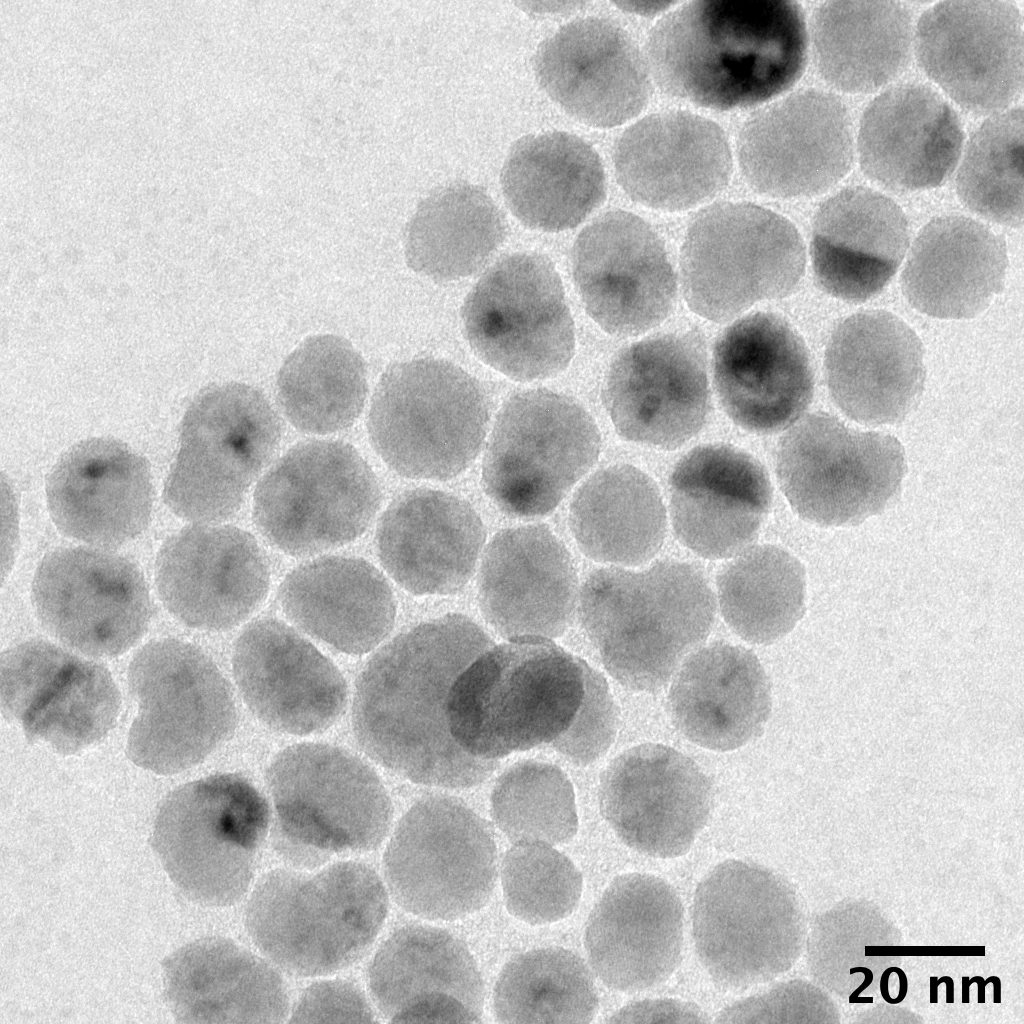
\includegraphics[width=\linewidth]{images/temh20.png}
	\end{subfigure}
\caption[TEM images of iron oxide nanoparticle]{TEM images of the iron oxide nanoparticles. From left to right: 5\,nm 10\,nm and 20\,nm nominal size in two different magnifications each (rows).}
\label{fig:tem}
\end{figure}
.


SAXS measurements of the prepared nanoparticle polymer foils where performed at the SSRL beamline 1-5. Samples were measured at 12\,keV for at two different spots for 5\,min each and averaged, a subtraction of the polymer matrix background was performed and a size distribution of spherical particles with hardsphere interaction was fitted to the radial profile. The low-q area is dominated by aggregate formation, which cannot be precisely quantified due to stray light and limited measuring range and is accounted for by a guinier-porod function, see \fref{fig:saxsps}  and  \fref{fig:saxspmma} \cite{percus1958,feigin1987,Ilavsky2009}.
The measurements do not show a clear and significant difference between the two polymer matrices. According to the regressions, the aggregates seem to have a radius of gyration of 20-30\,nm (the straylight limits the measurement validity in those small q areas), the porod $P$ of 2.5-3.8 suggests a dimensionality of the aggregates between 2 and 3.  \cite{feigin1987,lili2005}. The radii of the form factor agree within the corresponding margin of error with the values of determined by TEM measurements, the difference between the radius parameters of the structure factors and the form factor is most likely caused by the thin layer of oleic acid ligands between aggregating particles.


\begin{figure}[tp]
	\centering
	\begin{subfigure}[b]{0.3\textwidth}
		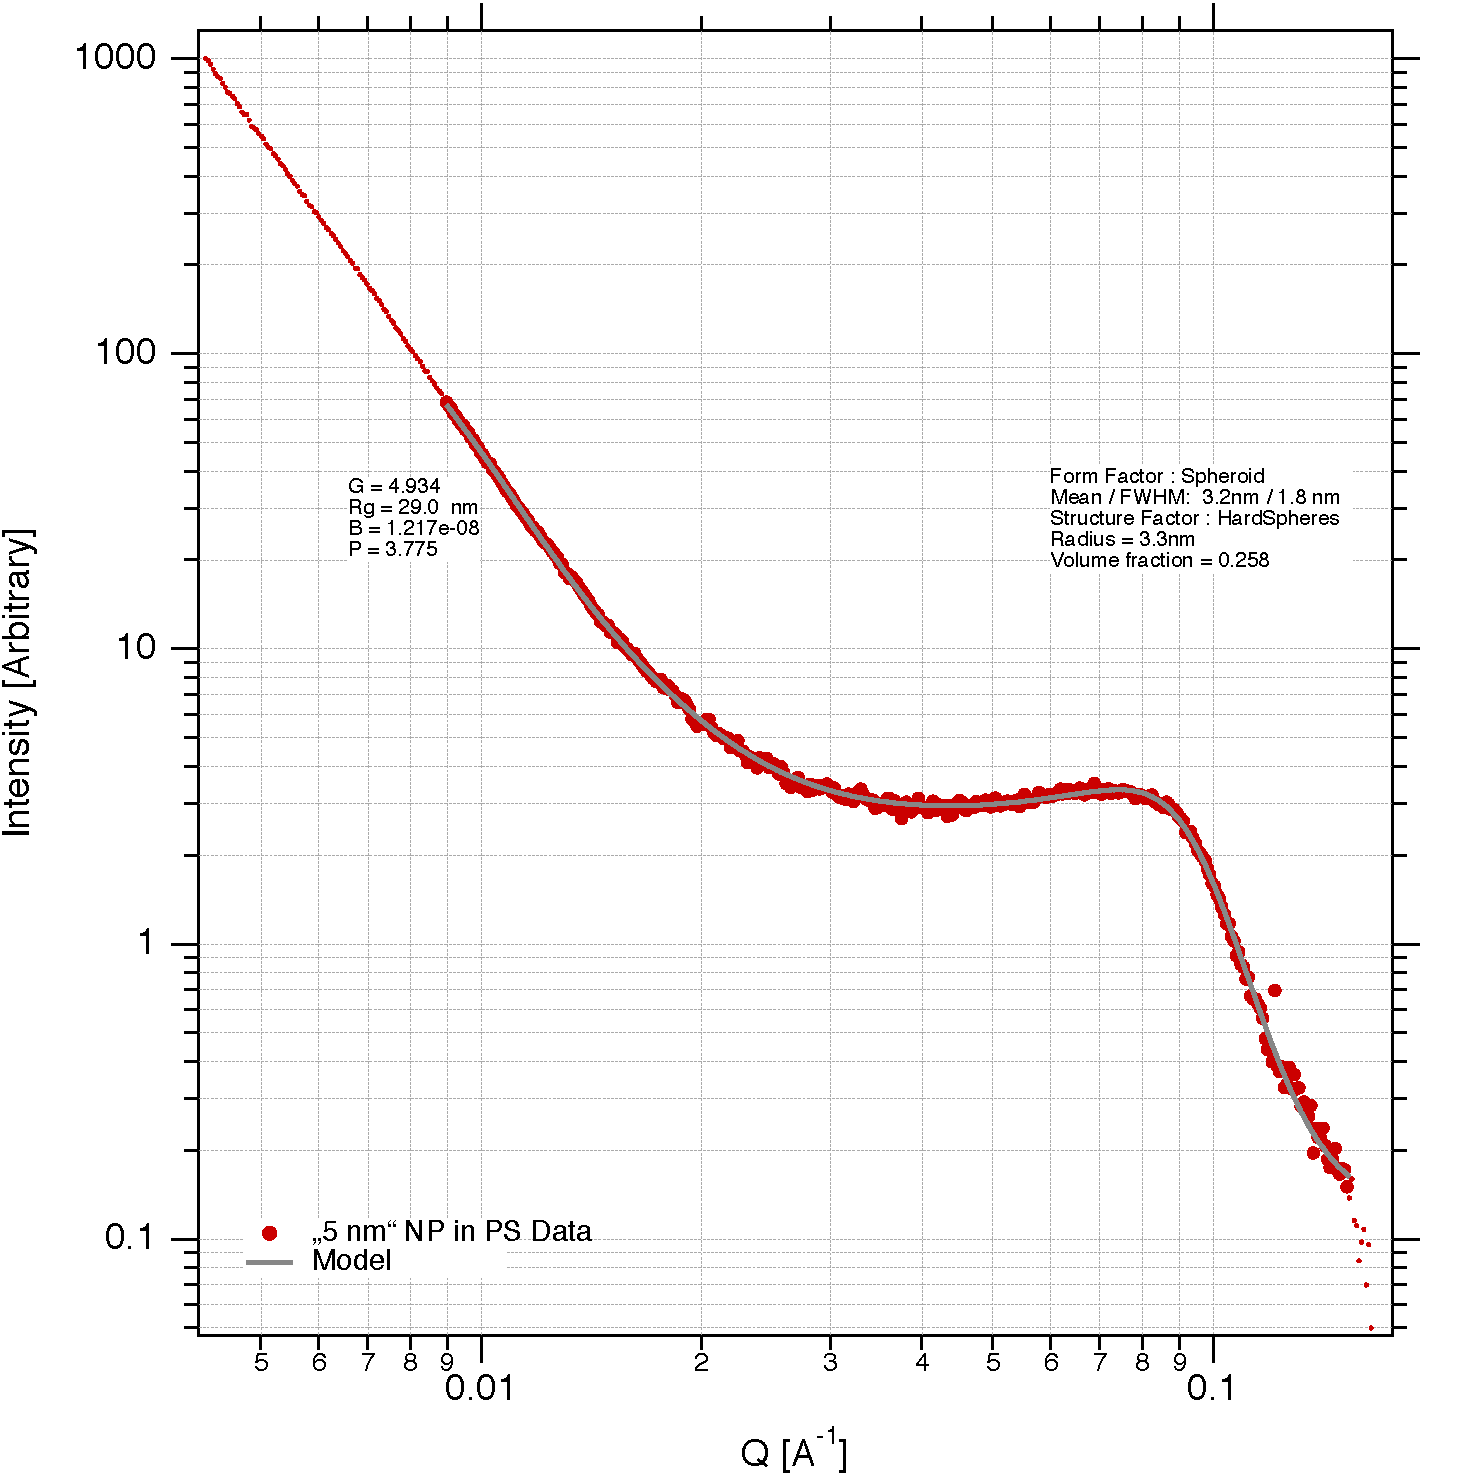
\includegraphics[width=\linewidth]{images/ps5.pdf}
	\end{subfigure}
	\begin{subfigure}[b]{0.3\textwidth}
		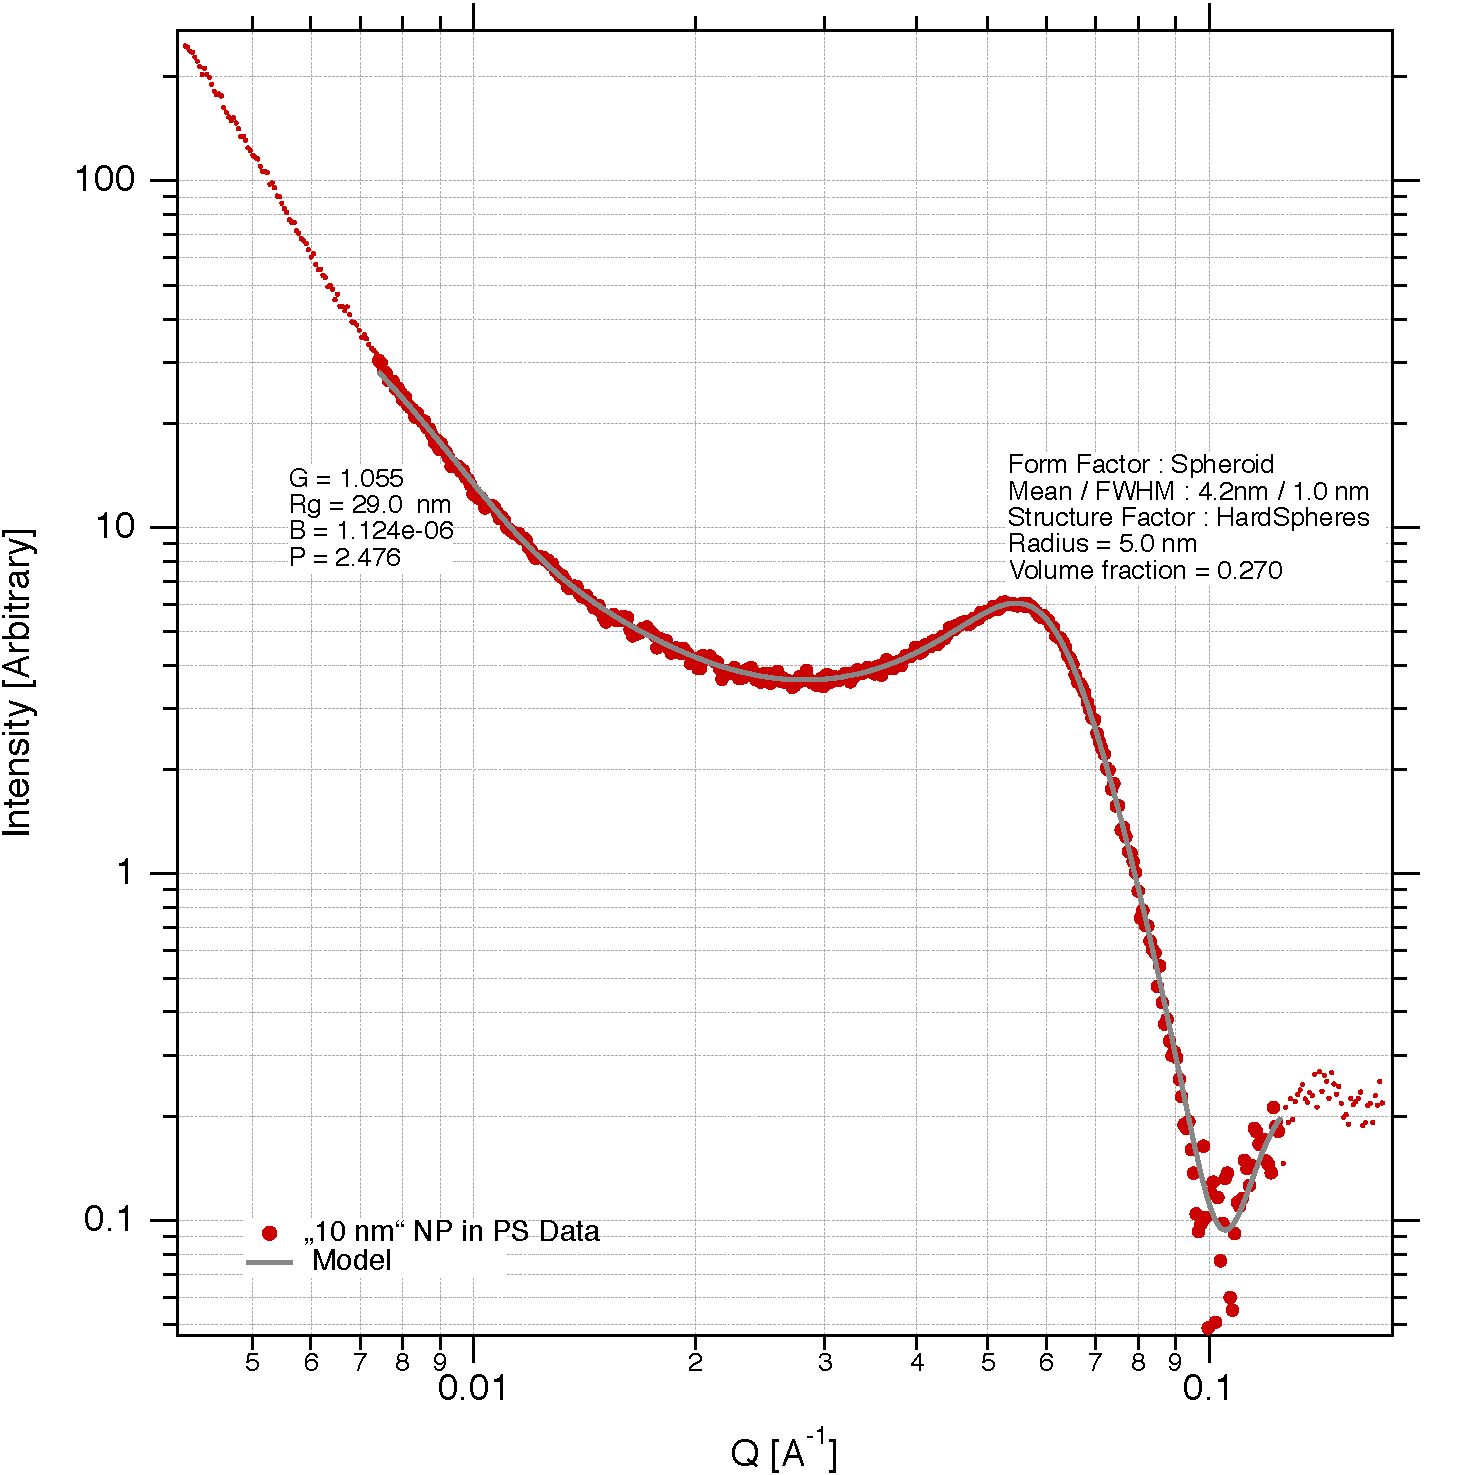
\includegraphics[width=\linewidth]{images/ps10.pdf}
	\end{subfigure}
	\begin{subfigure}[b]{0.3\textwidth}
		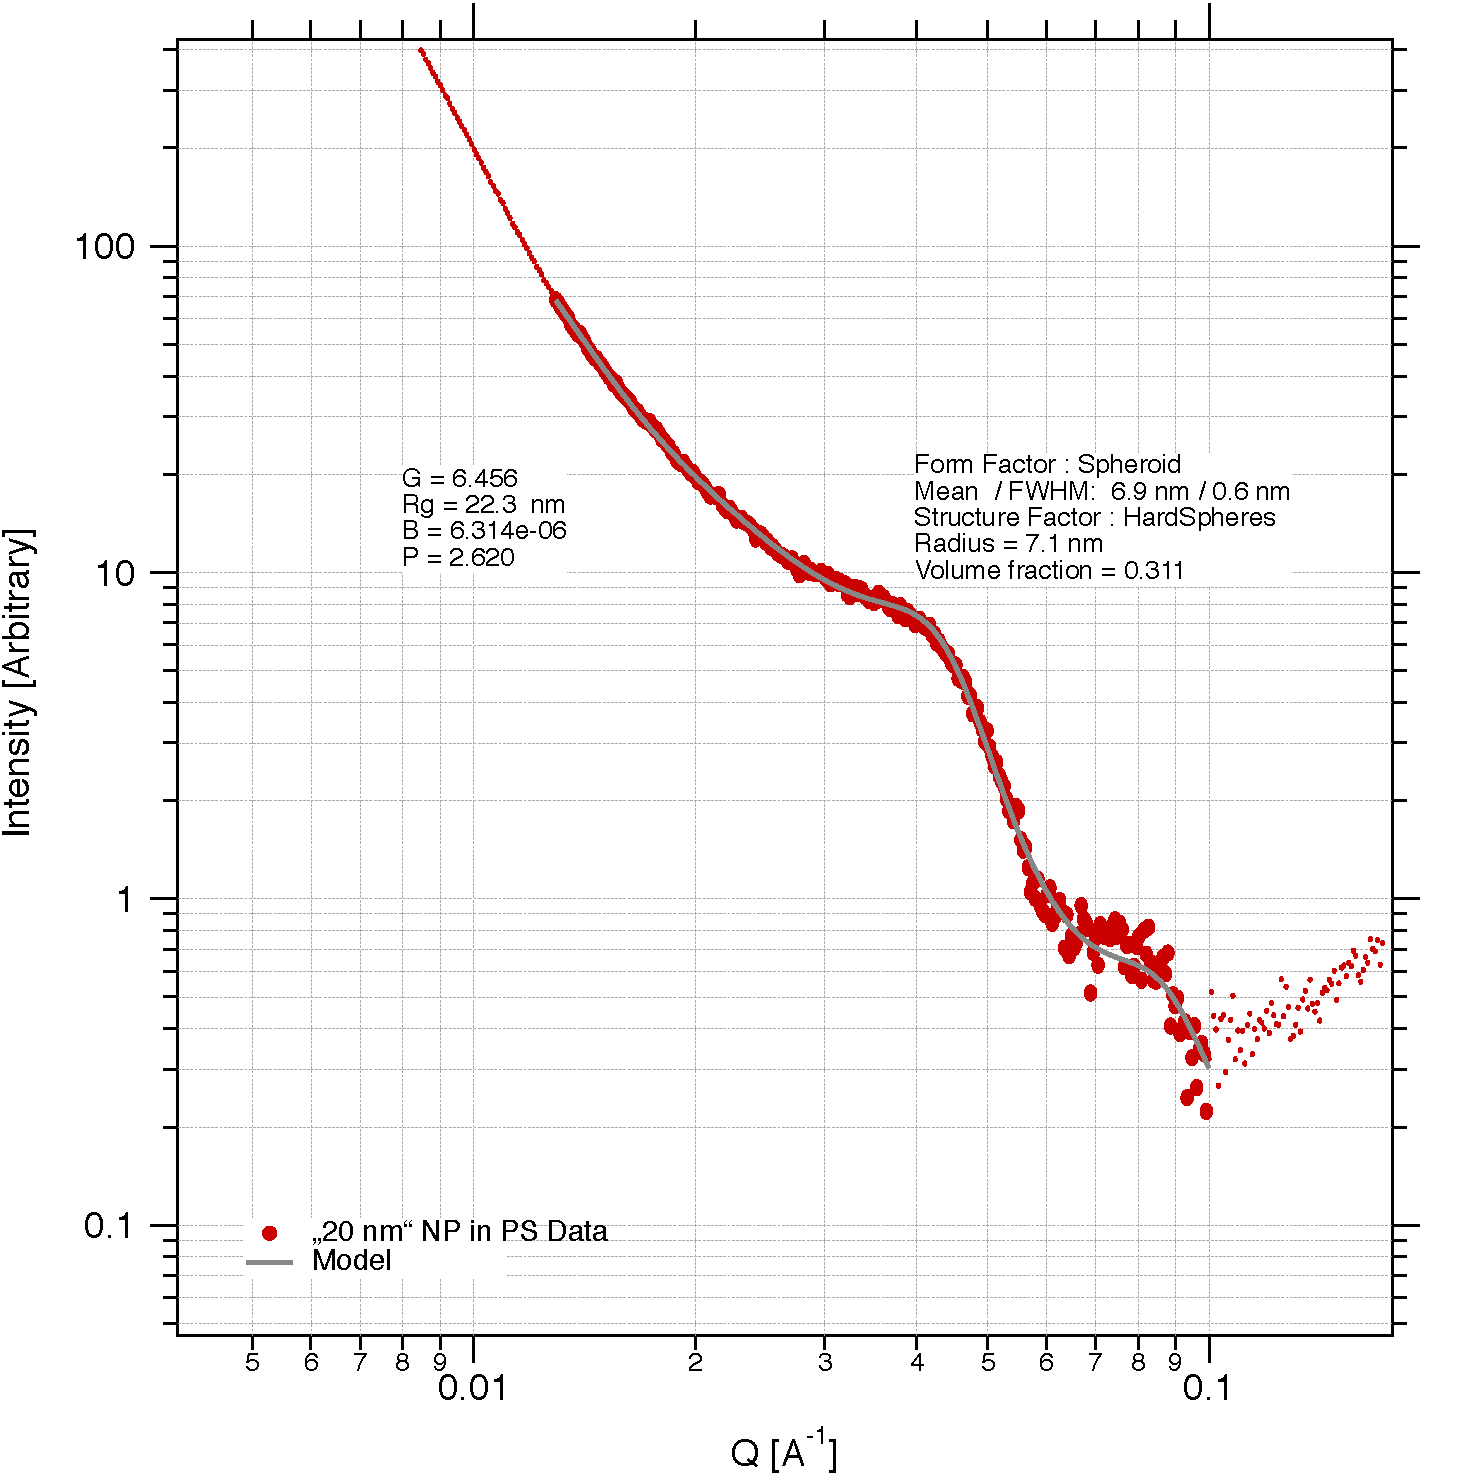
\includegraphics[width=\linewidth]{images/ps20.pdf}
	\end{subfigure}

	\caption[SAXS profile of iron oxide nanoparticles in polystyrene matrix]{SAXS profiles of nominal 5\,nm, 10\,nm and 20\,nm iron oxide nanoparticles in polystyrene matrix (left to right).}
	\label{fig:saxsps}
\end{figure}
\begin{figure}[tp]
	\centering
	\begin{subfigure}[b]{0.3\textwidth}
		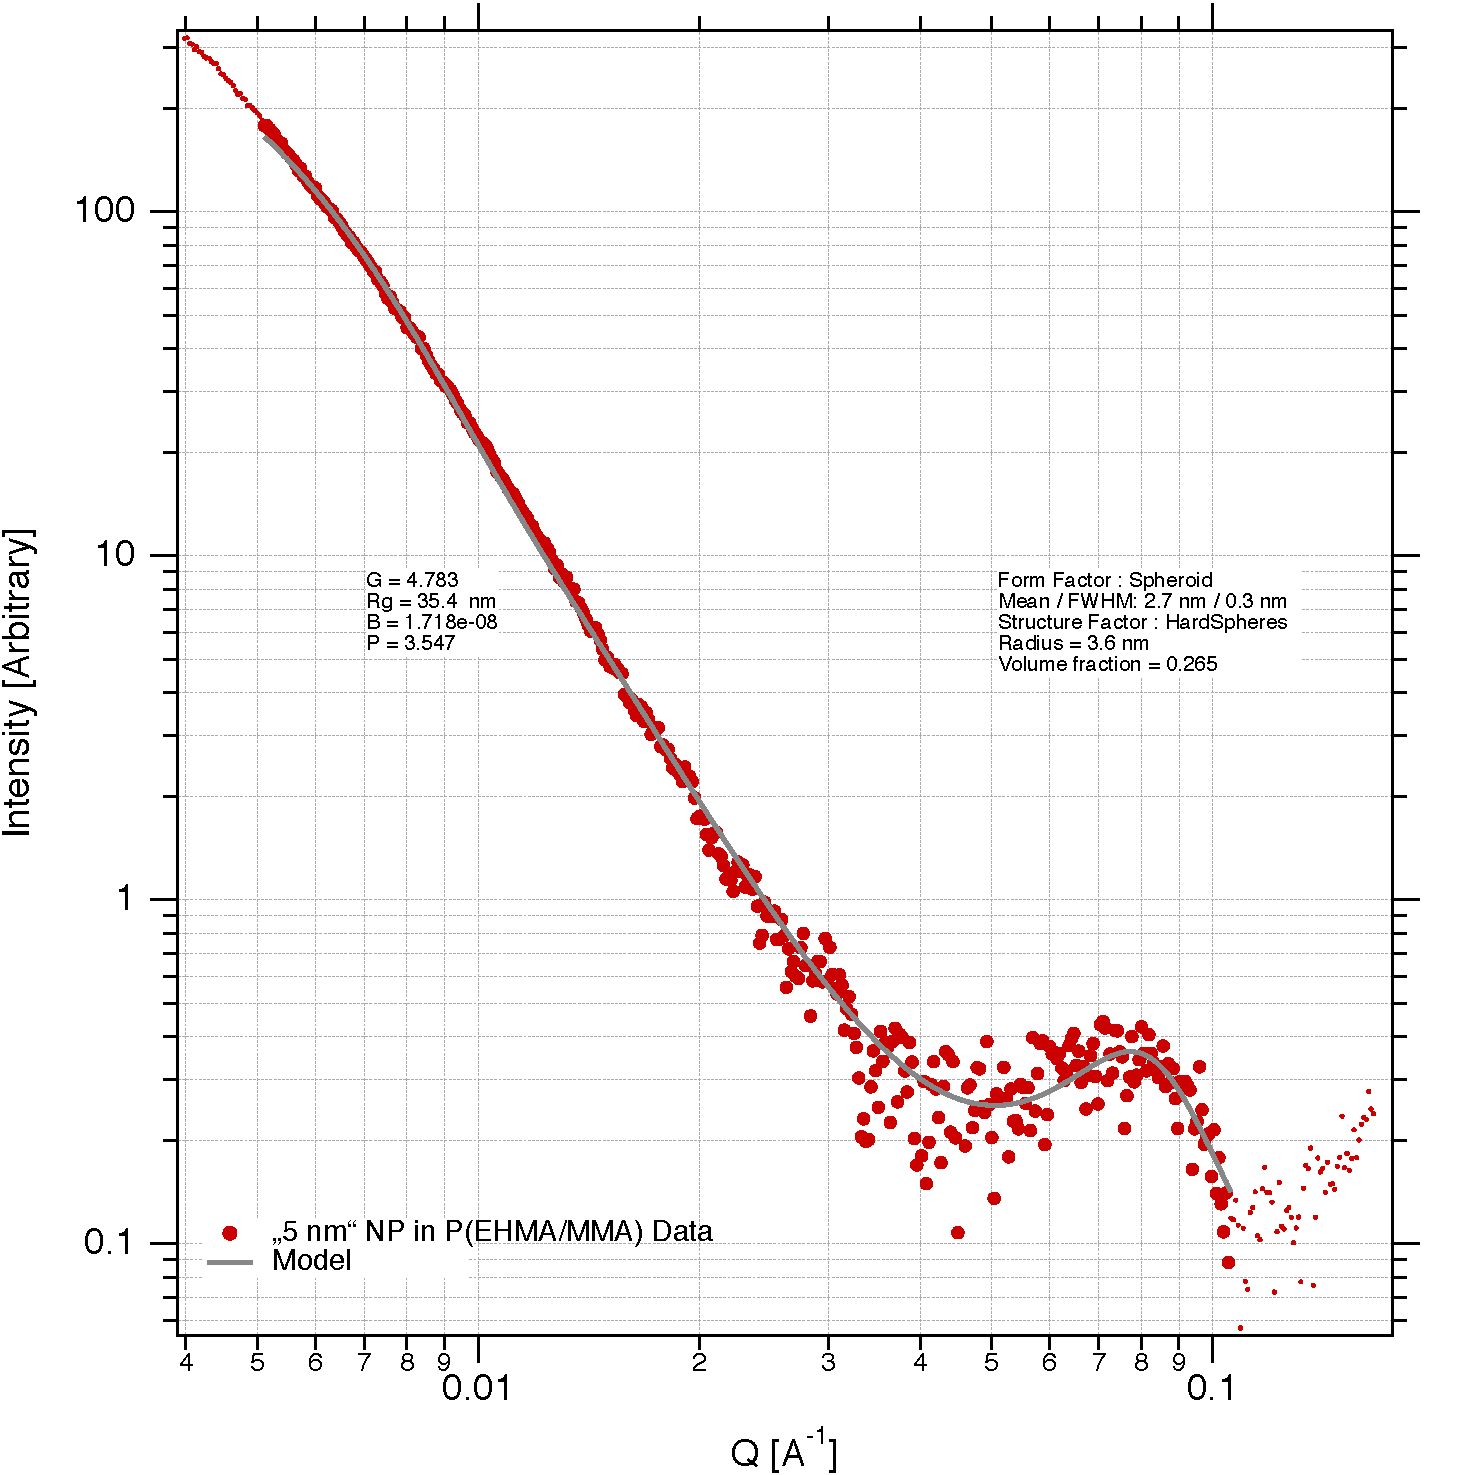
\includegraphics[width=\linewidth]{images/pmma5.pdf}
	\end{subfigure}
	\begin{subfigure}[b]{0.3\textwidth}
		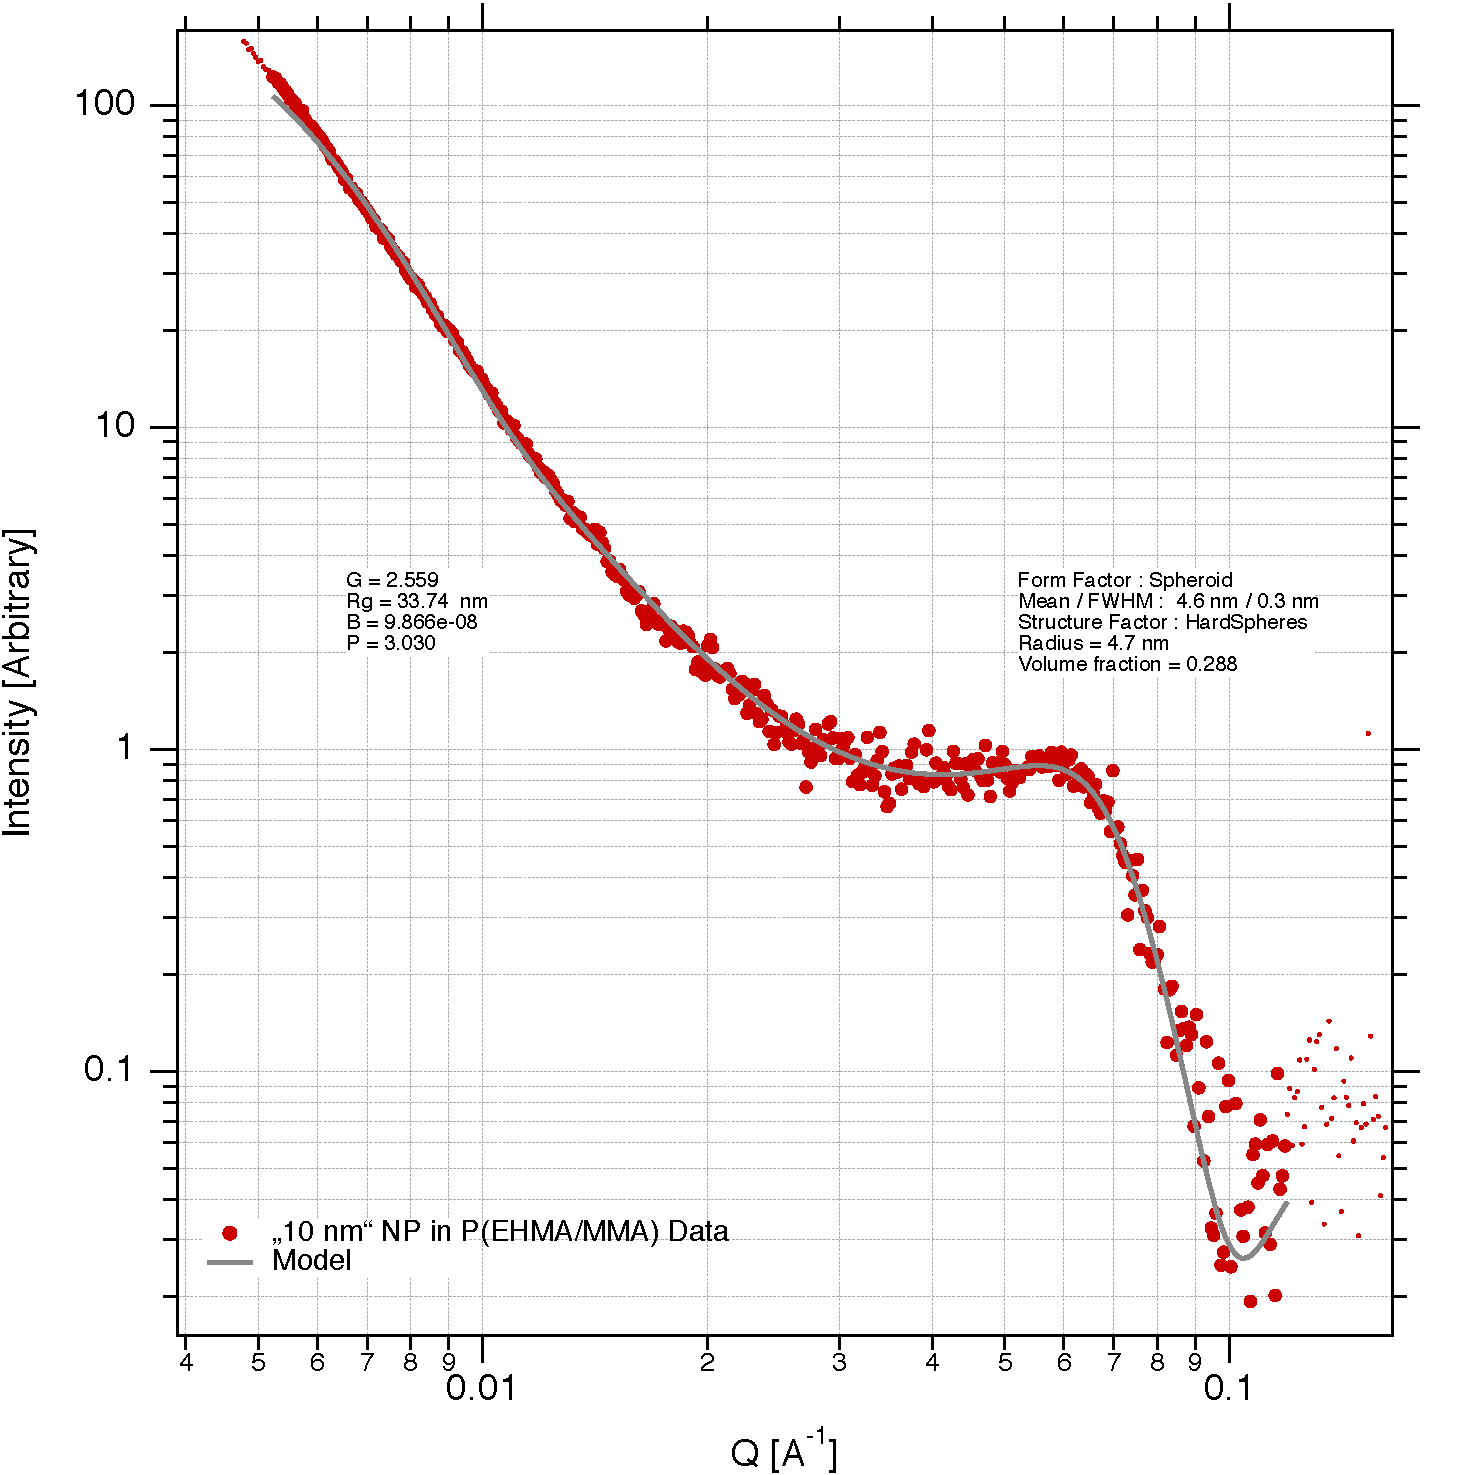
\includegraphics[width=\linewidth]{images/pmma10.pdf}
	\end{subfigure}
	\begin{subfigure}[b]{0.3\textwidth}
		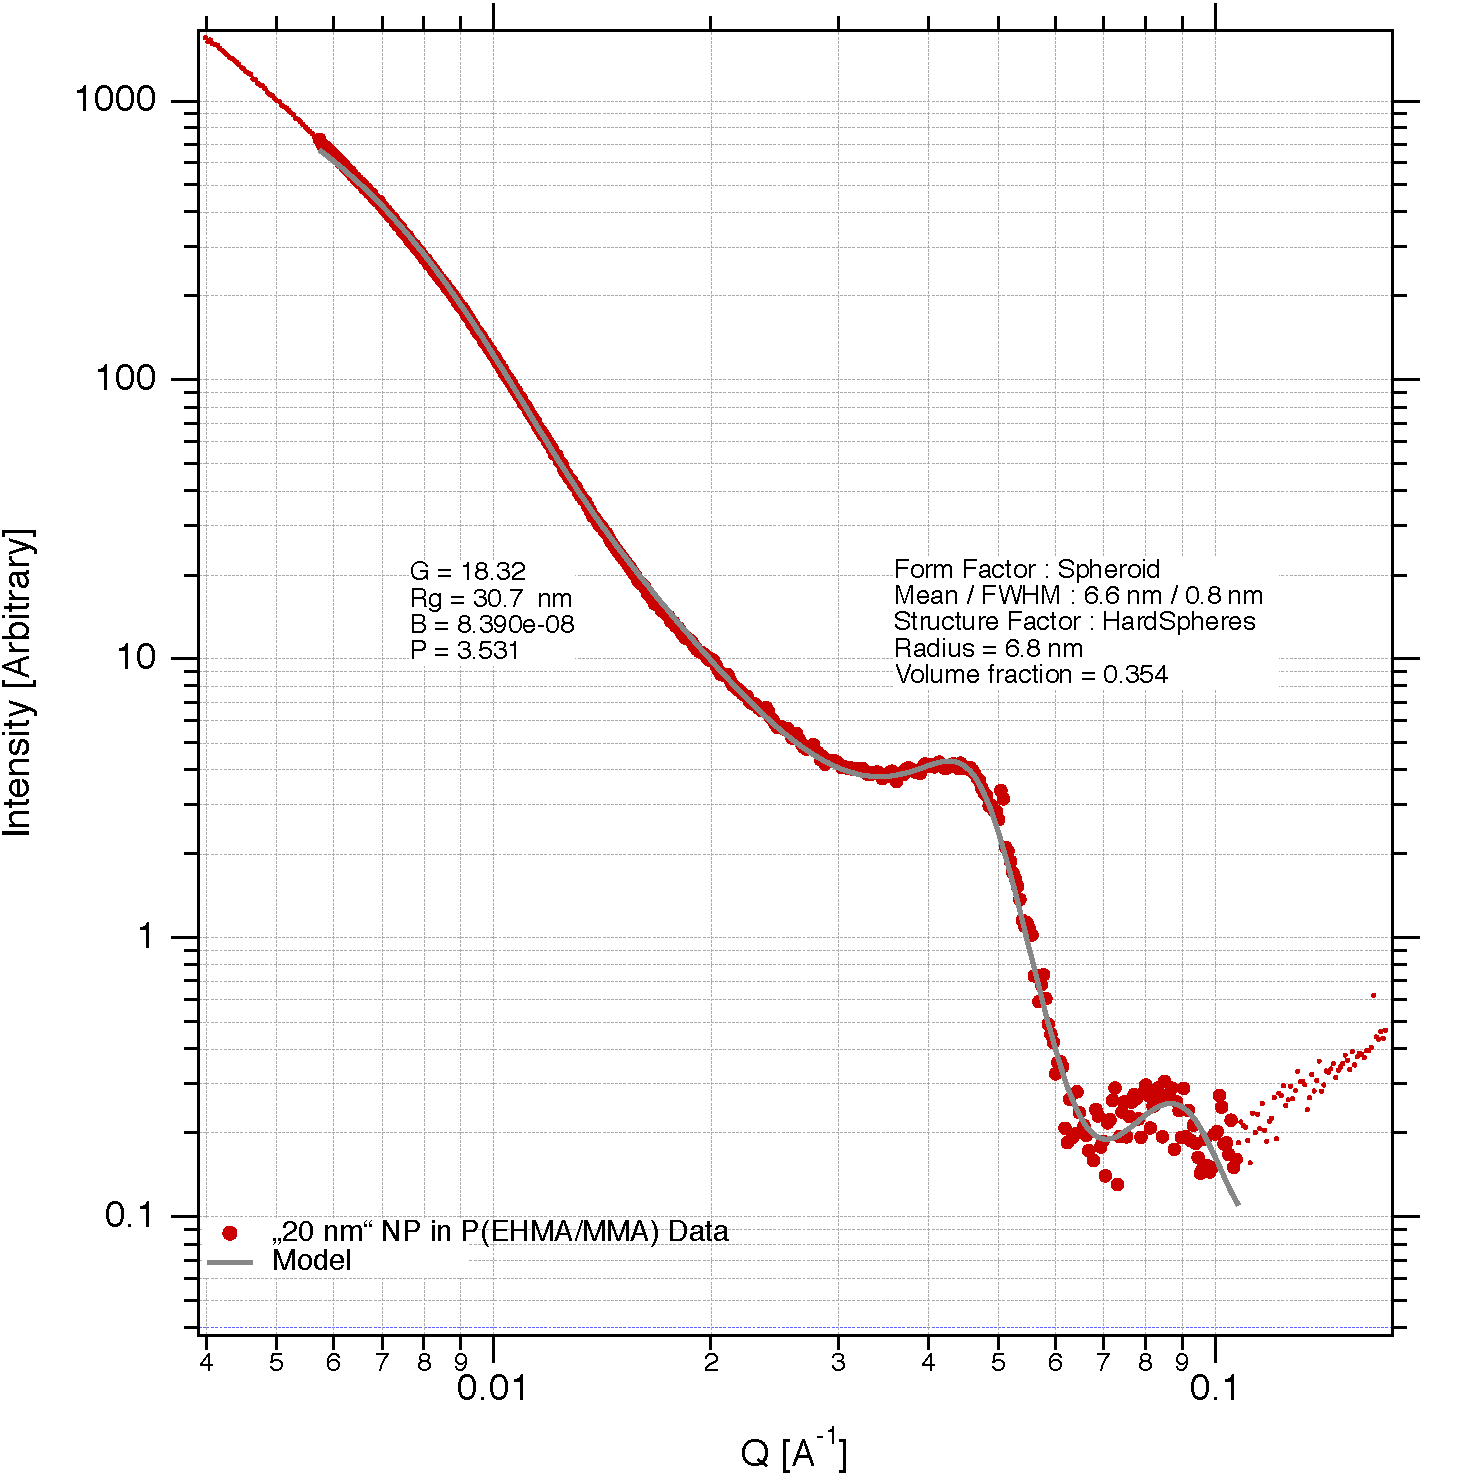
\includegraphics[width=\linewidth]{images/pmma20.pdf}
	\end{subfigure}
	
	\caption[SAXS profile of iron oxide nanoparticles in  Poly-(EHMA/MMA) matrix]{SAXS profiles of nominal 5\,nm, 10\,nm and 20\,nm iron oxide nanoparticles in Poly-(EHMA/MMA) matrix (left to right).}
	\label{fig:saxspmma}
\end{figure}

The SAXS measurements give a reasonably good insight into the expected results of the IDI scheme measurement of the same sample, which will differ due to the iron specificity and the smaller focal volume in the latter.  

\subsection{GaAs Crystal Films}
As a crystalline sample GaAs was chosen for its simple fcc structure and large product of the gallium K-shell fluorescence Energy and lattice constant. The samples were prepared by Ben Reeves at the Stanford Nanofabrication Facility. 
Using MOCVD, 50\,nm GaAs, 400\,nm AlGaAs as an etch stop and finally a 5\,um GaAs film were grown on an epi-ready (100)±0.1° GaAs substrate. The speciman was cut into 12\,mm\,x\,15\,mm pieces, each glued to an approx. 100\,um thick fused silica cover slip with the 5\,um film layer facing towards the silica. The substrate and the AlGaAs layer were selectively etched away via C6H8O7:H2O2 and HF:H2O wet etches, respectively. This left 5\,um thin GaAs films glued onto the the quartz slides (see \fref{fig:gaas_sample}).  XRD with Cu K-alpha was used to measure the width of the (004) GaAs bragg peak as 0.004°, indicative of high quality single crystals. 

\begin{figure}[tp]
	\centering
	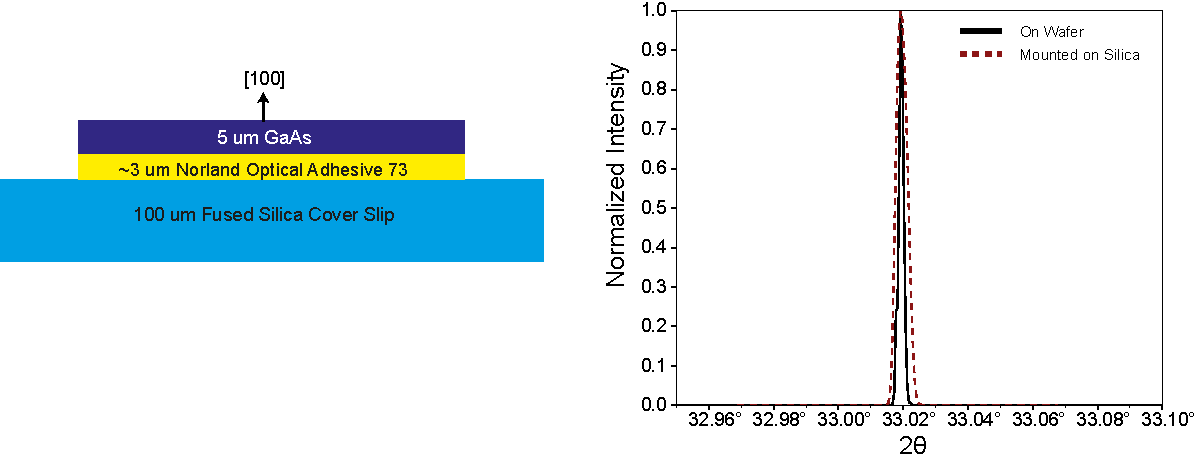
\includegraphics[width=0.8\linewidth]{images/gaas_sample.pdf}
	\caption[GaAs Sample]{Sketch of the GaAs single crystal glued to a fused silica cover slip and Cu-K$\alpha$ XRD measurement of the GaAs (004) reflex, showing a single crystal. After mounting on the cover slip, the peak is slightly broadened, most likely by an slighly uneven thickness of the glue layer. }
	\label{fig:gaas_sample}
\end{figure}


\section{Setup}
The setup used at EH5 at SACLA is shown in \fref{fig:setup}. 

The sample was mounted in an XXX angle to the beam on an XXX axis stage to allow scanning of the sample, ensure perpendicularly of the scanning directions to the beam to stay within the Rayleigh length of approx. XXX\,um while also ensuring a parallel alignment of the sample surface to one of the detectors. Overall, two MPCCD detectors were used: A Dual detector with two tiles, each 512x1024 pixels perpendicular to the FEL beam in a distance of 1\,m and a Short Working Distance Octal detector, consisting of eight 512x1024 tiles, parallel to the sample surface in a distance $d_{octal}$ ranging from XXX to XXX cm. To supress absorption and more importantly, air scattering, a vacuum pipe with Kapton windows was installed in between the sample and the Dual detector
An L-shaped aluminum plate was installed to reduce stray light as well as to allow mounting of the beamstop and filters to suppress coherent scattering and K$\beta$ fluorescence and between sample and detector.
\begin{figure}
	\centering
	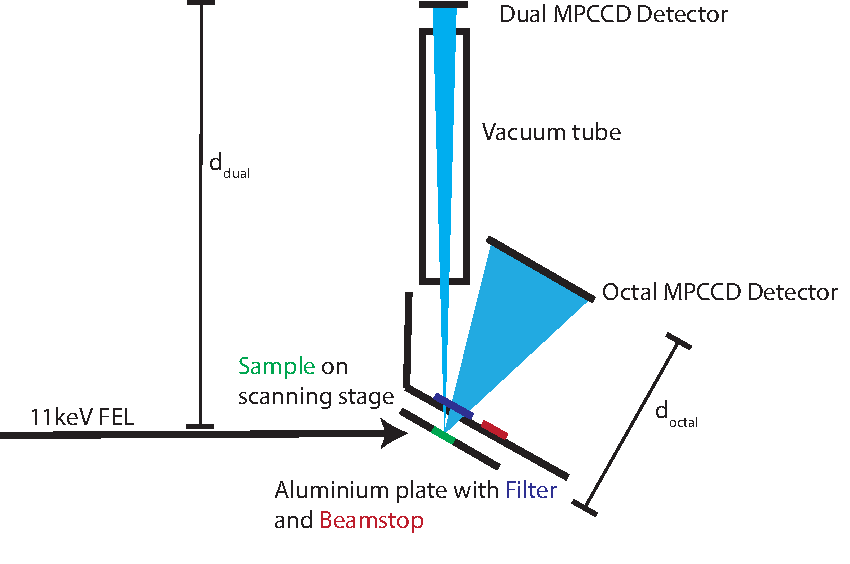
\includegraphics[width=0.8\linewidth]{images/setup.pdf}
	\caption[Experimental setup at SACLA]{Experimental setup at SACLA: The sample is mounted on a scanning stage and aligned to stay in focus during the scan and be parallel to the Octal MPCCD detector, which is in a distance $d_{octal}$. The angle between incoming FEL and Sample is XXX. Behind the sample, a stray light filter, beamstop and (depending on the sample) a filter foil is installed. The Dual detector is mounted $d_{dual}$=1\,m away from the sample in a XXX angle. To reduce air scattering, a vacuum tube is installed in the path from sample to Dual.}
	\label{fig:setup}
\end{figure}
\paragraph{Imaging the Focus}
The image to focus, 
\paragraph{Imaging Nanoparticles}
\paragraph{Imaging Crystals}

\section{Data Processing}
As the amount of recorded data is huge, an efficient strategy for filtering on shots, preprocessing the data to eliminate interferences and finally reconstruction has to be implemented.
\subsection{Shot filtering}
\subsection{Preprocessing}



\begin{figure}[tp]
	\centering
	\begin{subfigure}[b]{0.45\textwidth}
		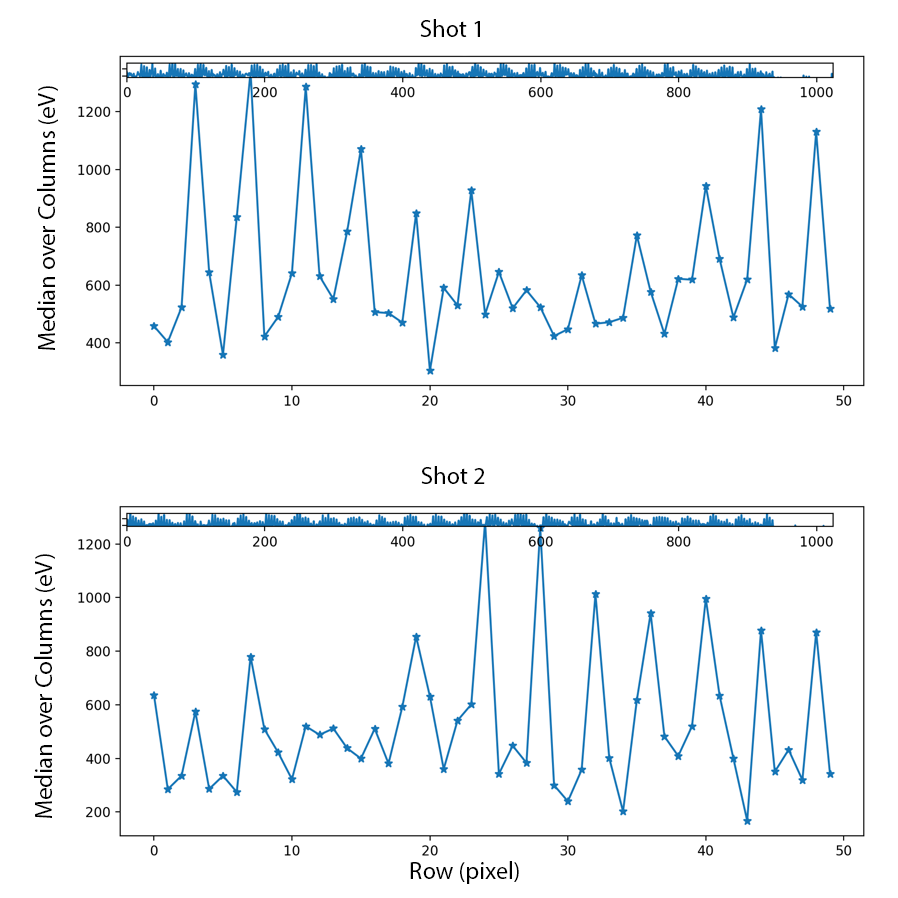
\includegraphics[width=\linewidth]{images/octalissue2.png}
	\end{subfigure}
	\begin{subfigure}[b]{0.45\textwidth}
		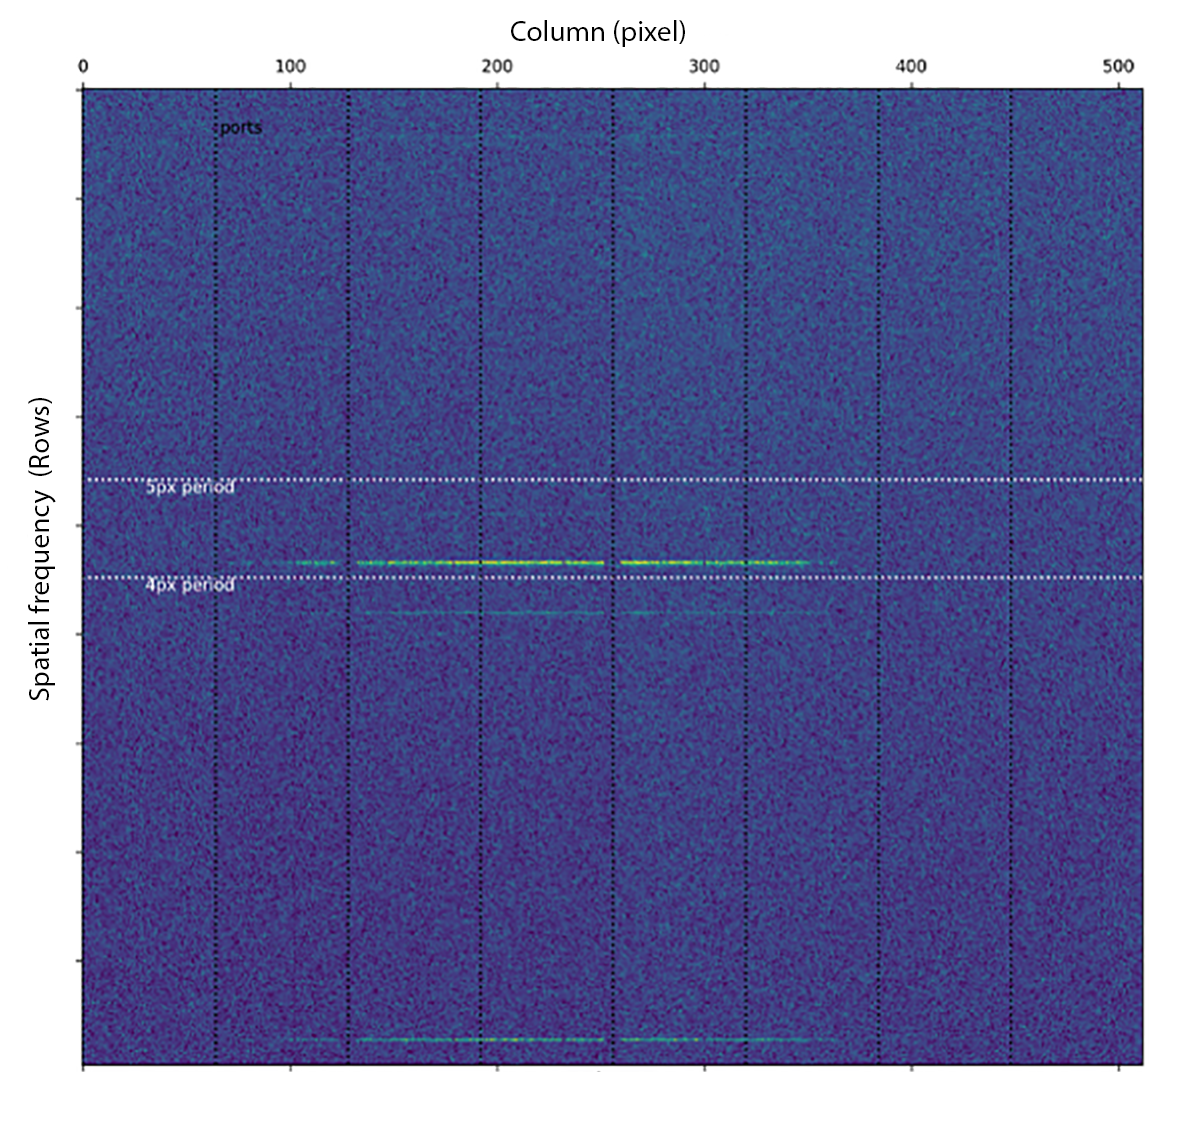
\includegraphics[width=\linewidth]{images/octalissue.png}
	\end{subfigure}

	\caption[Periodic noise on octal detector]{Periodic noise on octal detector after background subtraction: For two exemplary shots the median over columns of one detector tile is shown. A periodic noise is visible. The mean spatial spectrum (over the rows) for each column of the tile is shown on the right. The periodic noise is not uniformly affecting all the columns of the tile.}
	\label{fig:octalissue}
\end{figure}



\begin{figure}
	\centering
	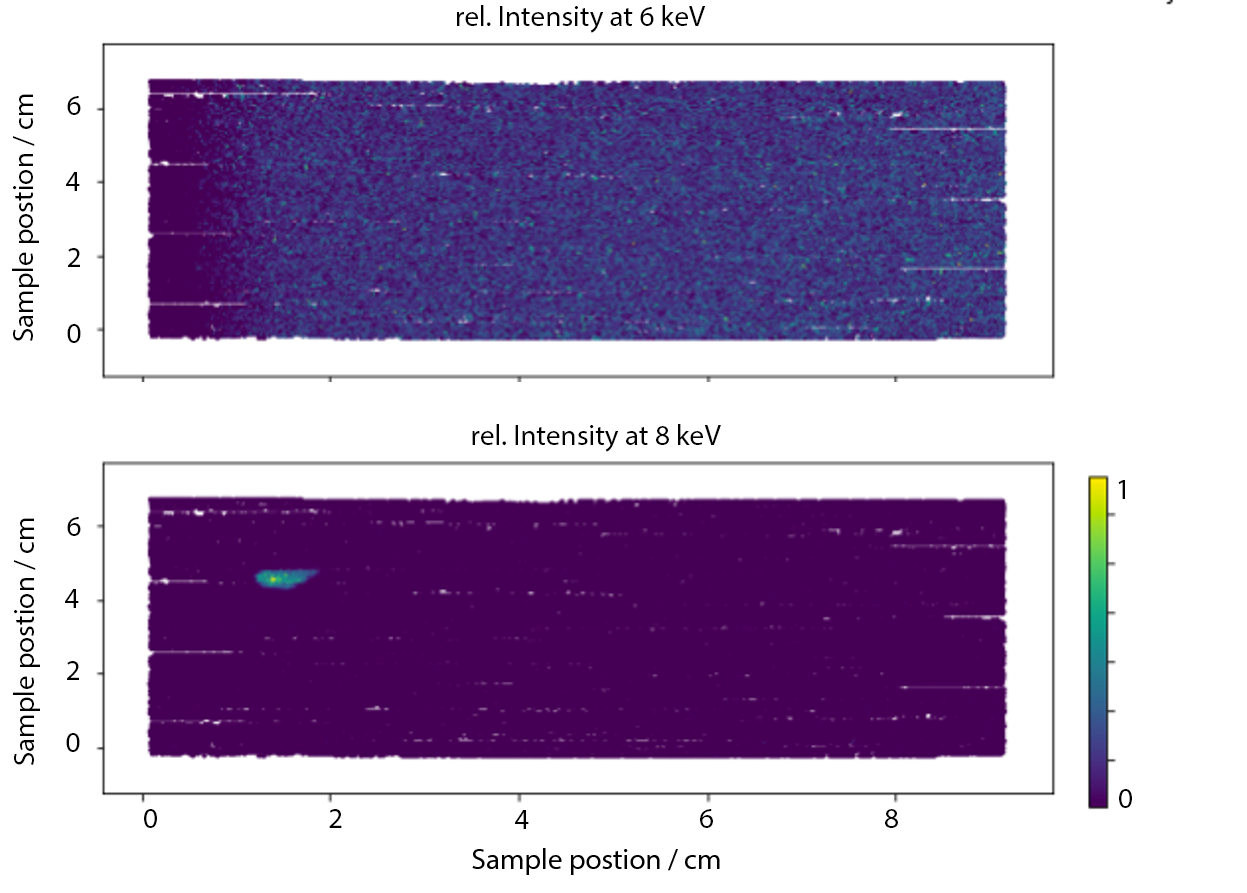
\includegraphics[width=0.7\linewidth]{images/xrf.png}
	\caption[Exemplary relative intensity of the 6 keV and 8 keV photon peak on the detector for different scanning positions on the sample]{Exemplary relative intensity of the 6 keV and 8 keV photon peak on the detector for different scanning positions on the sample. In this iron sample, a localized impurity, most likely copper, is clearly visible and can be masked out .}
\end{figure}

\begin{figure}
	\centering
	\begin{subfigure}{0.2\textwidth}
		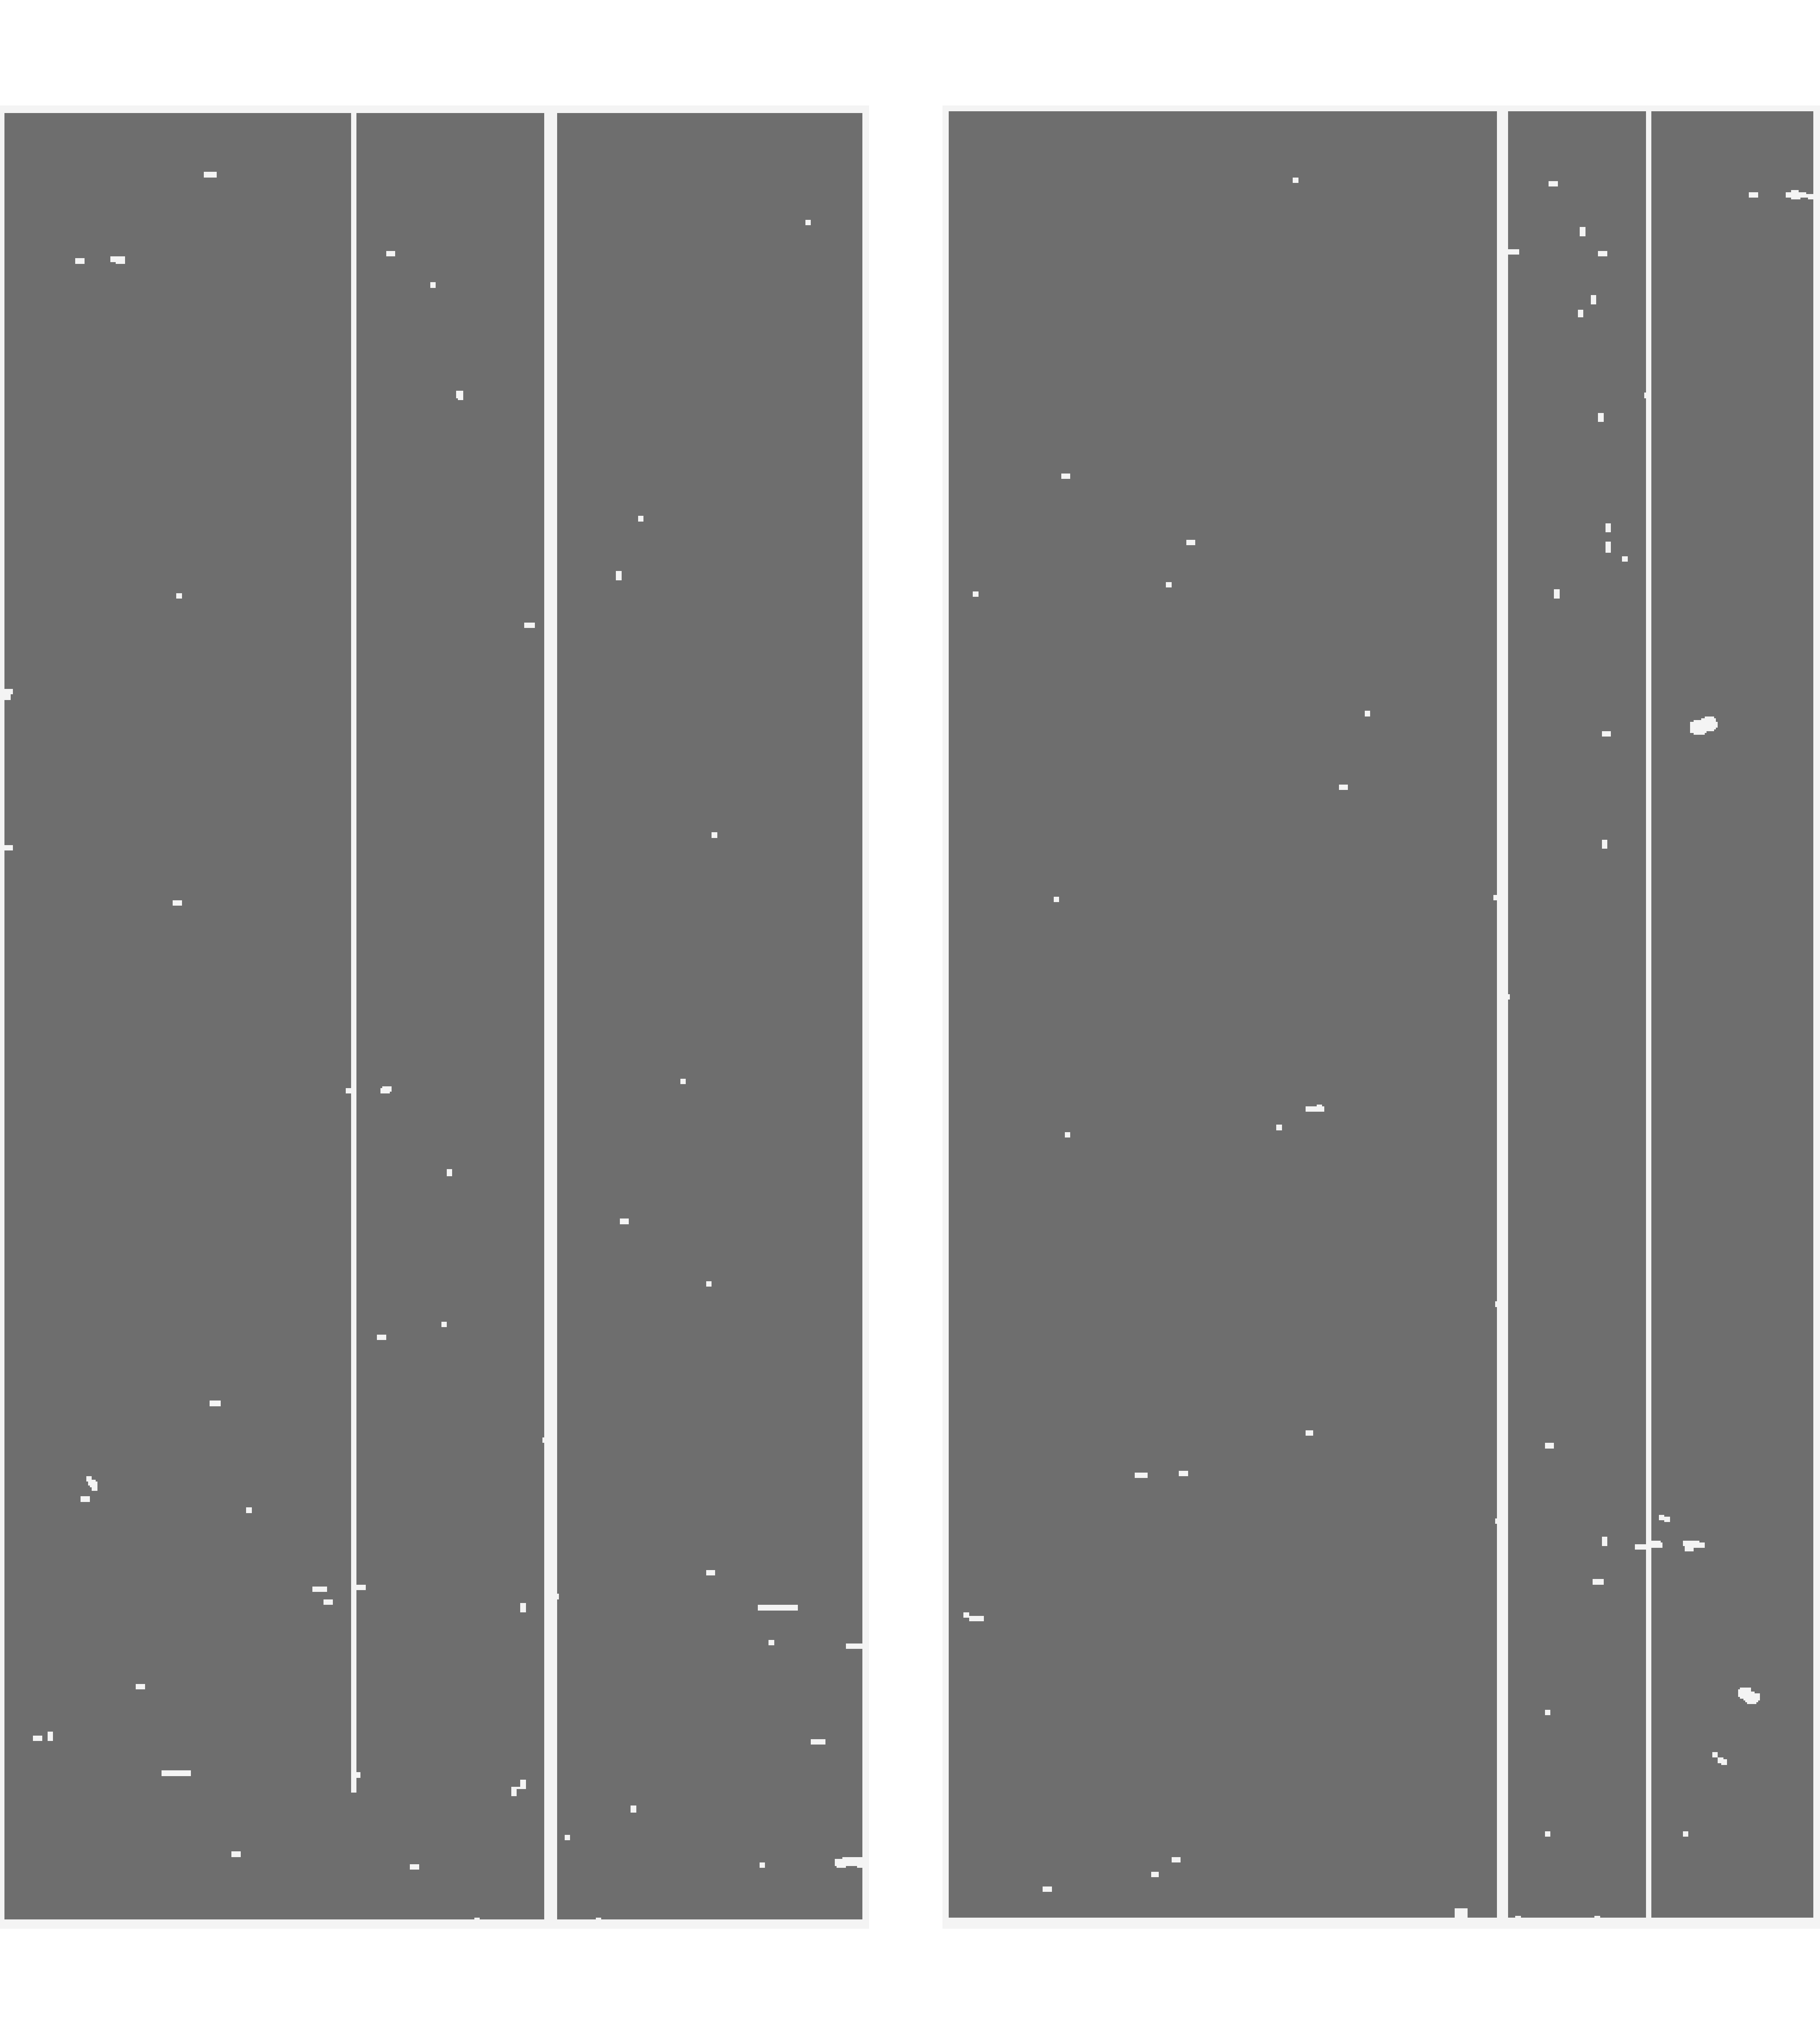
\includegraphics[width=\linewidth]{images/mask_dual.png}
	\end{subfigure}
	\hspace{1cm}
	\begin{subfigure}{0.2\textwidth}
		
\includegraphics[width=\linewidth]{images/mask_octal.png}
	\end{subfigure}
	\caption[Usable detector area]{Usable detector area (gray) of the dual (left) and octal (right) detector after signal correction and statistical filtering. Only the intersection of good areas for each run will be used. This way the same mask and number of correlation pairs will be used for samples that will be compared to each other.}	
\end{figure}

\paragraph{Shot filtering}

\paragraph{Filtering by sample position}
\paragraph{Detector masking}

\paragraph{Photon counting}



As shown in \fref{fig:spectrum}, the background corrected and masked spectrum of the detector shows peaks at multiplex of the fluorescence and excitation energy with a FWHM of .... . 


As discussed in \fref{chap:simulation}, the number of fluorescence photons can be estimated...


% Raw Data
% Spectrum
% Peaks


\paragraph{Crystal orientation}
For determining the relative orientation of the crystal with regards to the detector, Kossel lines as described in \fref{chap:kossel} can be used.  A semi-automatic alignment program was developed (\fref{fig:kosselfit}) and used the find the crystal orientation (\fref{tab:kosselfit}). As initial parameters, 5.65\,\AA\, lattice constant, 9.25\,keV energy and 800\,px detector distance and the result of a simple 2D cubic fit for the values of the translational shift were used. 
\begin{figure}
	\centering
	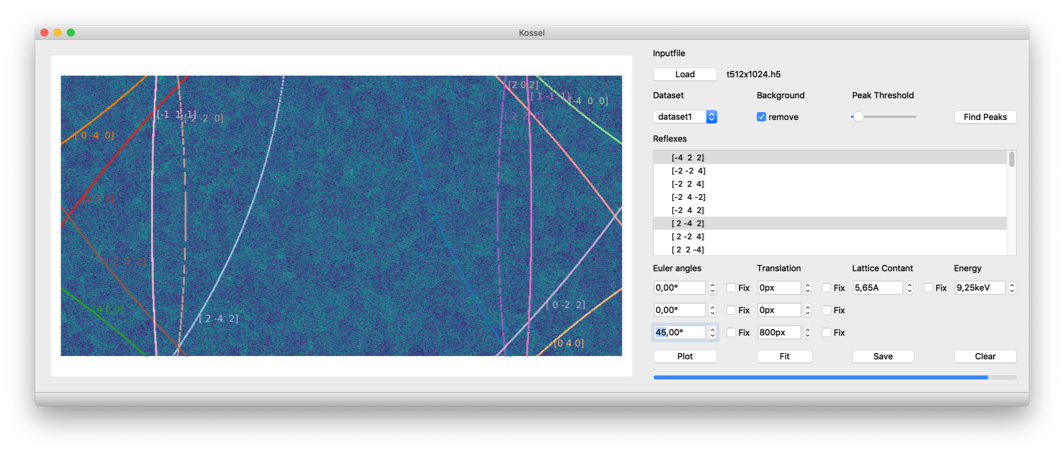
\includegraphics[width=0.8\linewidth]{images/kosselfit.png}
	\caption{Program for fitting Kossel lines to experimental data}
	\label{fig:kosselfit}
\end{figure}

\subsection{Reconstruction}




\section{Results}
\subsection{Imaging the Focus}
\subsubsection{Filtering}

\subsection{Imaging Nanoparticles}
\subsubsection{Filtering}
\subsection{Imaging Crystals}



\begin{table}[]
	\caption{Results of the Kossel line analysis}
	\begin{tabular}{lllll}
		\hline
		Sample & Initial Translation & Initial Rotation    & Energy & Rotation           \\
		& x,y in pixels      & Euler angles x,y,z & in keV    & Euler angles x,y,z \\
		\hline
		GaAs 1 &                    &                    &        &                    \\
		GaAs 2 &                    &                    &        &                   \\
		\hline
	\end{tabular}

\label{tab:kosselfit}
\end{table}
